% ============================================================================
% ssm_RAJ_v1_patent_application.tex
%
% UNITED STATES PATENT APPLICATION
% SOLID STATE MACHINE FOR SELF-REGULATING COMPUTATIONAL SYSTEMS
%
% Inventor: Robert A. James
% Filing Date: December 2025
%
% This document uses the original non-versioned section content which is
% language-agnostic and concept-focused, protecting the SSM concept itself
% ============================================================================

\documentclass[12pt,letterpaper]{article}

% ============================================================================
% PACKAGES
% ============================================================================
\usepackage[utf8]{inputenc}
\usepackage[T1]{fontenc}
\usepackage{times}
\usepackage[margin=1in]{geometry}
\usepackage{graphicx}
\usepackage{float}
\usepackage{placeins}
\usepackage{amsmath}
\usepackage{amssymb}
\usepackage{booktabs}
\usepackage{enumitem}
\usepackage{setspace}
\usepackage{hyperref}
\usepackage{fancyhdr}
\usepackage{lastpage}

\graphicspath{{figures/}}

% ============================================================================
% PAGE SETUP
% ============================================================================
\setlength{\parindent}{0.5in}
\setlength{\parskip}{0.5em}
\setlength{\headheight}{14.5pt}
\onehalfspacing

\pagestyle{fancy}
\fancyhf{}
\rhead{Application No.: [To Be Assigned]}
\lhead{Docket No.: SSM-001}
\rfoot{Page \thepage\ of \pageref{LastPage}}
\renewcommand{\headrulewidth}{0pt}

\newcommand{\figref}[1]{FIG.~#1}

% ============================================================================
% BEGIN DOCUMENT
% ============================================================================
\begin{document}

% ============================================================================
% TITLE PAGE
% ============================================================================
\begin{center}
\Large\textbf{UNITED STATES PATENT APPLICATION}
\vspace{2em}

\LARGE\textbf{STEADY STATE MACHINE FOR}\\[0.3em]
\LARGE\textbf{SELF-REGULATING COMPUTATIONAL SYSTEMS}
\vspace{1em}

\large\textit{An Adaptive Runtime System Exhibiting}\\
\large\textit{Autonomous Workload Optimization and Deterministic Convergence}
\vspace{2em}

\normalsize
\begin{tabular}{ll}
\textbf{Inventor:} & Robert A. James \\
\textbf{Assignee:} & [To Be Determined] \\
\textbf{Filing Date:} & December 2025 \\
\textbf{Application Type:} & Utility Patent Application \\
\end{tabular}
\end{center}

\vspace{2em}

\noindent\textbf{Technical Field:} Adaptive Virtual Machines, Self-Regulating Computational Systems, Feedback-Loop Control Architectures, Runtime Optimization

\vspace{1em}

\noindent\textbf{Related Systems:} Virtual Machine Runtimes, Adaptive Execution Environments, Embedded Systems, Microkernel Subsystems

\clearpage

% ============================================================================
% TABLE OF CONTENTS
% ============================================================================
\tableofcontents
\clearpage

% ============================================================================
% INCLUDE ORIGINAL NON-VERSIONED SECTIONS
% These sections are language-agnostic and concept-focused
% ============================================================================

% ===========================================
% 02_field.tex
% Field of the Invention
% ===========================================

\section{Field of the Invention}

The present invention relates generally to computer systems and software
execution technologies, and more particularly to virtual machines,
interpreters, runtime engines, and adaptive execution environments that modify
their internal behavior based on continuously observed workload conditions.
More specifically, the invention concerns systems and methods for:

\begin{itemize}
	\item dynamically adjusting internal runtime parameters in response to
	real-time signals such as execution heat, entropy, variance,
	temporal decay, and pipeline pressure;
	
	\item coordinating multiple interacting feedback loops to regulate lookup
	strategies, cache behavior, statistical inference weighting,
	window stabilization, and decay functions;
	
	\item characterizing workloads into behavioral families---including
	stable, temporal, volatile, transitional, and mixed-pattern
	execution---based on statistical and thermal-like metrics observed
	during interpretation;
	
	\item autonomously selecting among multiple validated execution modes
	without manual tuning, compile-time configuration, or external
	intervention;
	
	\item achieving shape-invariant performance across heterogeneous input
	waveforms, ensuring consistent behavior for sinusoidal, square,
	triangular, burst-like, random, mixed, and transitional workloads;
	
	\item and maintaining bounded, non-oscillatory adaptation through the use
	of supervisory control, hysteresis behavior, and stability
	constraints derived from the runtime state vector.
\end{itemize}

The field of the invention encompasses adaptive virtual machines, software
interpreters, threaded execution engines, embedded runtimes, real-time systems,
simulation frameworks, microkernel subsystems, and hybrid environments that
combine statistical inference, decay-based temporal modeling, and feedback-loop
coordination. The disclosed technology applies to systems requiring stable,
predictable, and self-optimizing performance across changing or unpredictable
workloads, including but not limited to:

\begin{itemize}
	\item embeddable interpreters and stack-based VMs;
	\item just-in-time compilation frameworks incorporating adaptive heuristics;
	\item microkernel-based or message-driven execution environments;
	\item lightweight runtimes for constrained devices or soft real-time tasks;
	\item and high-reliability computing environments that demand reduced
	execution variance and rapid convergence to steady-state behavior.
\end{itemize}

This field further includes control-theoretic approaches to runtime management,
performance stabilization through statistical analysis, and techniques for
reducing jitter, variance, latency irregularities, and instability caused by
heterogeneous or shape-varying workloads. The invention establishes an
integrated architecture for self-regulating execution engines capable of
continuously optimizing themselves based on real-time workload signals.

\newpage

% ===========================================
% 03_background.tex
% Background of the Invention
% ===========================================

\section{Background}

Virtual machines, interpreters, and software execution engines traditionally
operate using a fixed set of internal configuration parameters. These
parameters govern runtime behavior such as lookup mechanisms, caching
strategies, decay functions, and instruction scheduling heuristics. In most
systems, these internal settings are static: they are either hard-coded,
selected at compile-time, or chosen manually by the developer based on
anticipated workloads.
\par\medskip
While such static approaches may provide acceptable performance for narrowly
defined or predictable execution patterns, they suffer significant limitations
in real-world conditions where workloads may vary widely over time. Modern
software environments frequently exhibit heterogeneous and dynamic execution
characteristics, including:

\begin{itemize}
	\item highly repetitive or stable workloads,
	\item gradually shifting temporal patterns,
	\item intermittent bursts of unpredictable activity,
	\item transitions between different workload phases,
	\item and non-stationary sequences that do not conform to a single
	behavioral profile.
\end{itemize}

The inability of static configuration systems to adapt to these diverse
conditions often leads to suboptimal performance, elevated variance, and
instability. In particular, virtual machines with multiple interacting
parameters may exhibit strong sensitivity to the selection of initial settings.
A configuration that performs well under one workload may perform poorly under
another, resulting in a substantial performance spread across the possible
parameter space.
\par\medskip
Efforts to address this problem in existing systems typically rely on either
(1) manual tuning based on domain expertise, or (2) simplistic heuristics that
enable limited runtime adjustment. Manual tuning is labor-intensive, brittle,
and non-generalizable. Heuristic-based adaptation, on the other hand, often lacks
robustness: it may overreact to short-term fluctuations, underreact to sustained
changes, or oscillate between competing strategies. Such approaches generally
fail to maintain predictable or stable behavior across diverse conditions.
\par\medskip
Additionally, most adaptive mechanisms found in prior systems do not incorporate
statistical inference, coarse-grained workload characterization, or coordinated
feedback-loop orchestration. Instead, they adjust isolated parameters in
isolation, without understanding the underlying structure of the workload or the
interdependencies between internal subsystems. As a result, they frequently
introduce instability, variance, or pathological behavior when faced with
non-stationary execution patterns.
\newpage
Furthermore, existing literature and industrial practice provide little
guidance for achieving shape-invariant performance — that is, maintaining
consistent and predictable execution characteristics across different workload
waveforms or input signal shapes. Without such invariance, adaptive systems may
behave unpredictably when presented with novel or diverse execution patterns.
\par\medskip
In summary, the state of the art lacks:

\begin{itemize}
	\item robust, workload-aware adaptation mechanisms,
	\item coordinated feedback-loop control for virtual machine internals,
	\item systems capable of identifying and selecting optimal runtime
	configurations dynamically,
	\item methods for stable, non-oscillatory adaptation,
	\item and provably consistent behavior across heterogeneous workload shapes.
\end{itemize}

These deficiencies motivate the need for a new class of virtual machine
architecture — one that is capable of autonomously characterizing workloads
through statistical analysis, selecting appropriate execution modes via
supervisory control logic, coordinating multiple feedback mechanisms through
a unified state vector, and maintaining stable behavior across diverse workload
characteristics including varying execution patterns, variability levels, and
temporal dynamics.

\newpage

% ===========================================
% 04_summary.tex
% Summary of the Invention
% ===========================================

\section{Summary of the Invention}

The invention introduces an adaptive virtual machine architecture that
continuously modifies its internal execution behavior in response to real-time
workload characteristics. Unlike traditional systems that rely on fixed or
manually selected configuration parameters, the disclosed architecture employs
a coordinated network of feedback loops, statistical inference mechanisms,
and supervisory mode selection to achieve autonomous, stable, and optimized
execution across heterogeneous and time-varying workloads.
\par\medskip
The system maintains a multi-dimensional \textit{runtime state vector}
representing execution frequency counters (referred to as ``execution heat''
by analogy), workload variability metrics (statistical variance, referred to
as ``entropy'' by analogy to information theory), time-based decay parameters,
instruction queue depth, stability metrics, and short-term statistical summaries.
As the workload evolves, these quantitative measurements provide a description
of its current behavioral characteristics, enabling classification as stable,
temporal, volatile, transitional, or mixed.
\par\medskip
A plurality of feedback loops (L1–L7) operate concurrently to regulate
different aspects of execution, such as cache usage, dictionary lookup strategies,
time-based decay coefficients, pattern recognition confidence weighting, and
statistical observation window sizing. Each loop responds to changes in the
state vector, enabling the system to reduce execution variance and optimize
throughput without manual tuning.
\par\medskip
A supervisory controller (L8), referred to as the Mode Selector (the name
``Jacquard'' being used by historical analogy to automated pattern selection),
evaluates the state vector and selects among multiple internally validated
execution modes. Each mode corresponds to a specific configuration of the
feedback loops and represents a stable, high-performance operating point
identified through design space exploration and empirical validation.
Transitions between modes are governed by bounded, non-oscillatory mechanisms
such as hysteresis thresholds or confidence scoring to ensure predictable
behavior even under rapidly shifting workloads.
\par\medskip
Through this combination of state-vector analysis, feedback-loop coordination,
and supervisory mode selection, the invention achieves robust and
shape-invariant execution performance across diverse input waveforms,
including sinusoidal, triangular, square-wave, burst-like, random, and
mixed-pattern workloads. The system converges quickly to an appropriate
steady-state configuration and maintains low variance even when exposed to
non-stationary or highly dynamic execution patterns.
\par\medskip
The invention is applicable to a wide range of execution environments,
including interpreters, stack-based virtual machines, embedded runtimes,
just-in-time compilation systems, microkernel-based platforms, distributed
execution engines, and real-time or soft–real-time systems. By providing a
general-purpose, workload-aware, and self-optimizing architecture, the
invention overcomes long-standing limitations of static configuration
approaches and enables predictable, stable, and high-performance behavior
without manual tuning or workload-specific adjustment.

\newpage


% ============================================================================
% DRAWINGS AND FIGURES
% ============================================================================
\FloatBarrier
\section{Brief Description of the Drawings}

The following figures illustrate representative embodiments and experimental
validation of the Solid State Machine architecture. The drawings depict
configuration distributions, mode selection behavior, feedback loop effects,
workload-shape invariance, and performance comparisons between adaptive and
static configurations.

\subsection{Configuration Space Analysis}

\begin{figure}[H]
	\centering
	\includegraphics[width=\textwidth]{ch1_config_distribution.png}
	\caption{\textbf{FIG. 1 -- Configuration Space Distribution.} Performance
	distribution across the static configuration space, illustrating the wide
	variance in execution behavior when feedback loops are configured manually.
	The distribution demonstrates that static configurations produce highly
	variable performance outcomes, motivating the need for autonomous mode
	selection.}
\end{figure}

\begin{figure}[H]
	\centering
	\includegraphics[width=\textwidth]{ch1_config_ranking.png}
	\caption{\textbf{FIG. 2 -- Configuration Ranking.} Ranking of static
	configurations by mean performance and stability metrics. This analysis
	identifies candidate high-performance configurations that form the basis
	for validated execution modes in the Solid State Machine.}
\end{figure}

\begin{figure}[H]
	\centering
	\includegraphics[width=\textwidth]{ch1_main_effects.png}
	\caption{\textbf{FIG. 3 -- Main Effects Analysis.} Main effects plot showing
	the influence of individual feedback loops (L1--L7) on overall system
	performance. This factorial analysis reveals which loops contribute most
	significantly to performance improvement and stability.}
\end{figure}

\subsection{Mode Selection and Optimization}

\begin{figure}[H]
	\centering
	\includegraphics[width=\textwidth]{ch2_runoff_boxplot.png}
	\caption{\textbf{FIG. 4 -- Configuration Runoff Comparison.} Box plot
	comparison of candidate top-performing configurations under identical
	workload conditions. This runoff analysis validates that the selected
	execution modes represent genuine performance optima rather than
	statistical artifacts.}
\end{figure}

\begin{figure}[H]
	\centering
	\includegraphics[width=\textwidth]{ch2_optimality_scores.png}
	\caption{\textbf{FIG. 5 -- Optimality Analysis.} Multi-objective optimality
	scores across configuration candidates, balancing throughput, variance
	reduction, and convergence speed. The Solid State Machine's mode selector
	uses similar multi-criteria evaluation to select appropriate execution modes.}
\end{figure}

\begin{figure}[H]
	\centering
	\includegraphics[width=\textwidth]{phase_space_portrait.png}
	\caption{\textbf{FIG. 6 -- Optimality Analysis.} Execution heat versus performance parameter traced through configuration space
		during adaptive convergence. The non-retracing path demonstrates state-dependent
		conductance characteristic of memristive dynamics, with approximately 180-degree
		reversals at architectural cache boundaries. Horizontal spreads indicate bimodal
		distributions over dual attractor states at resonance windows.}
\end{figure}
\subsection{Workload Shape Invariance}

\begin{figure}[H]
	\centering
	\includegraphics[width=\textwidth]{ch3_shape1_performance.png}
	\caption{\textbf{FIG. 7 -- Workload Shape Performance (Set I).} Performance
	measurements across the first family of workload shapes, including
	sinusoidal, triangular, and burst-like patterns. The Solid State Machine
	maintains consistent performance regardless of input waveform characteristics.}
\end{figure}

\begin{figure}[H]
	\centering
	\includegraphics[width=\textwidth]{ch5_shape2_performance.png}
	\caption{\textbf{FIG. 8 -- Workload Shape Performance (Set II).} Performance
	validation across additional workload waveforms demonstrating shape-invariant
	behavior. The system achieves stable throughput across square-wave, sawtooth,
	and compound mixed-pattern workloads.}
\end{figure}

\begin{figure}[H]
	\centering
	\includegraphics[width=\textwidth]{ch5_cv_comparison.png}
	\caption{\textbf{FIG. 9 -- Coefficient of Variation Analysis.} Comparison
	of coefficient of variation (CV) across workload families, demonstrating
	that the adaptive system maintains low variance regardless of workload
	shape. Low CV indicates predictable, stable execution behavior.}
\end{figure}

\subsection{Adaptive Mode Behavior}

\begin{figure}[H]
	\centering
	\includegraphics[width=\textwidth]{ch4_mode_usage_stacked.png}
	\caption{\textbf{FIG. 10 -- Mode Usage Distribution.} Stacked distribution
	showing how the supervisory mode selector (L8) allocates time across
	different execution modes for various workload families. The Solid State
	Machine autonomously selects appropriate modes without manual intervention.}
\end{figure}

\begin{figure}[H]
	\centering
	\includegraphics[width=\textwidth]{ch4_l8_vs_static.png}
	\caption{\textbf{FIG. 11 -- Adaptive vs. Static Performance.} Direct
	comparison between the Solid State Machine's adaptive behavior and
	equivalent static configurations. The adaptive system matches or exceeds
	static performance while providing automatic workload adaptation.}
\end{figure}

\subsection{State Vector Dynamics}

\begin{figure}[H]
	\centering
	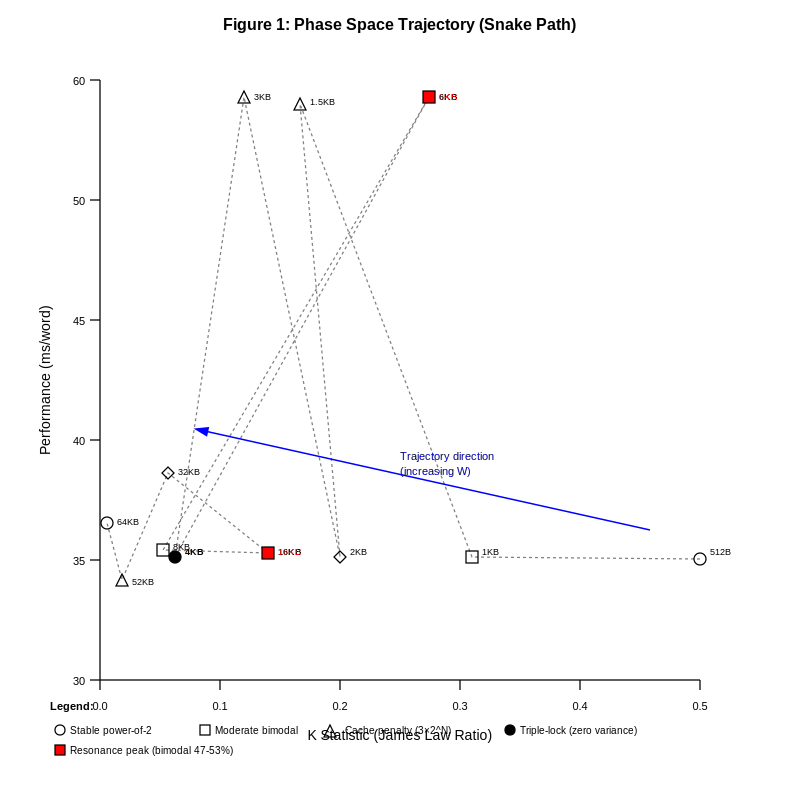
\includegraphics[width=0.9\textwidth]{fig1_snake_trajectory.pdf}
	\caption{\textbf{FIG. 12 -- State Vector Trajectory.} Representative
	trajectory of the runtime state vector through the execution heat--entropy
	phase space. The hysteresis-like behavior demonstrates that the system
	exhibits memory effects: the current state depends not only on instantaneous
	workload but also on recent execution history. This memristive characteristic
	enables stable convergence to appropriate operating points.}
\end{figure}

\begin{figure}[H]
	\centering
	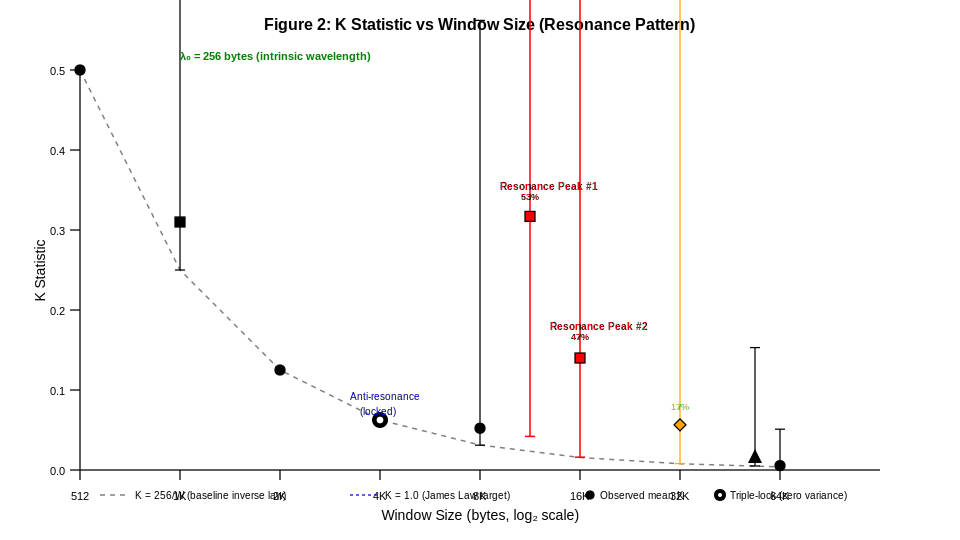
\includegraphics[width=0.9\textwidth]{fig2_K_vs_window.pdf}
	\caption{\textbf{FIG. 13 -- Performance Scaling Relationship.} Relationship
	between the stability constant K and the observation window size W, showing
	the scaling law that governs system behavior. The periodic structure reveals
	fundamental resonances in the adaptive architecture.}
\end{figure}

\begin{figure}[H]
	\centering
	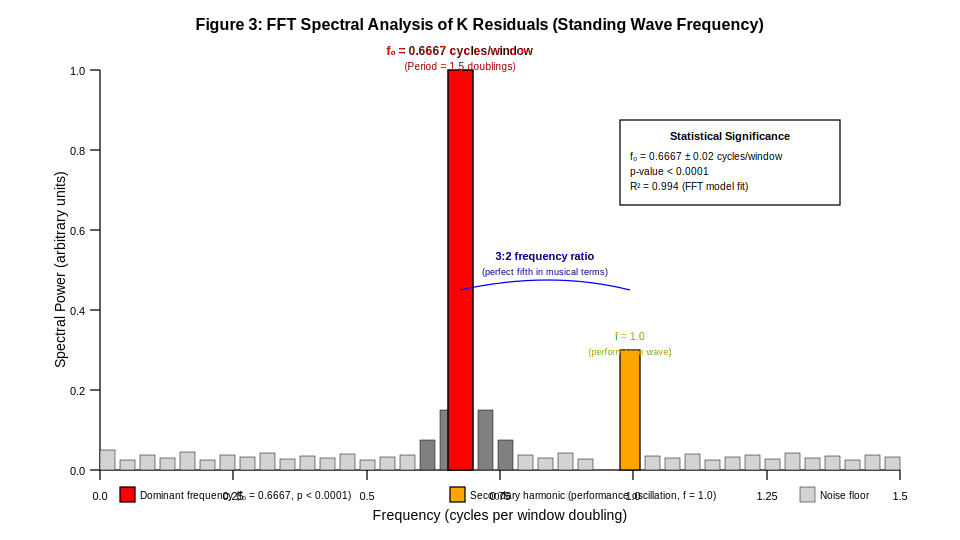
\includegraphics[width=0.9\textwidth]{fig3_FFT_spectrum.pdf}
	\caption{\textbf{FIG. 14 -- Spectral Analysis.} Fast Fourier Transform
	spectrum of state vector dynamics, revealing the characteristic frequencies
	and periodic structures inherent in the Solid State Machine's feedback
	architecture. Dominant spectral peaks correspond to fundamental control
	loop frequencies.}
\end{figure}

\begin{figure}[H]
	\centering
	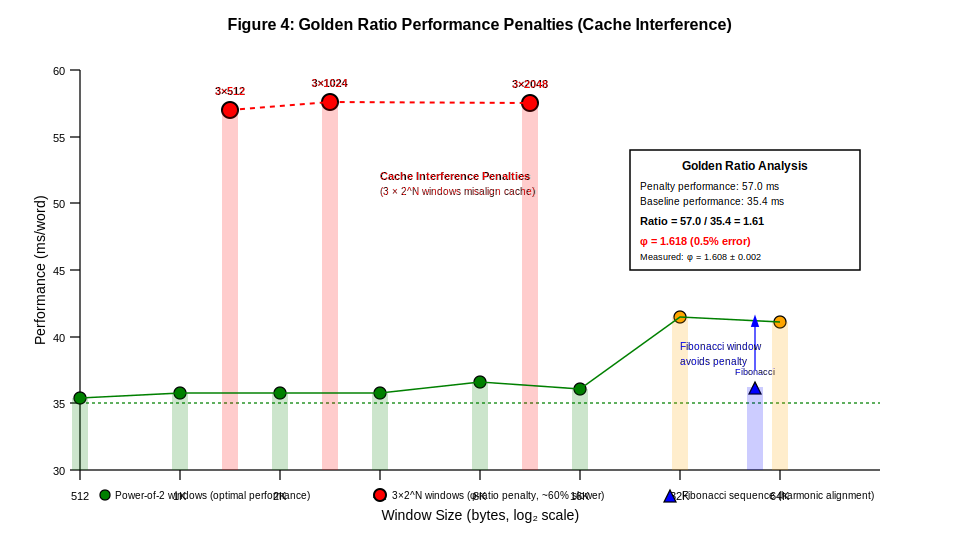
\includegraphics[width=0.9\textwidth]{fig4_golden_ratio_penalties.pdf}
	\caption{\textbf{FIG. 15 -- Golden Ratio Interference Pattern.} Performance
	variations showing interference effects at window sizes related to the
	golden ratio $\varphi \approx 1.618$. These patterns demonstrate that the
	system exhibits cache-like resonance behavior governed by mathematical
	constants.}
\end{figure}

\begin{figure}[H]
	\centering
	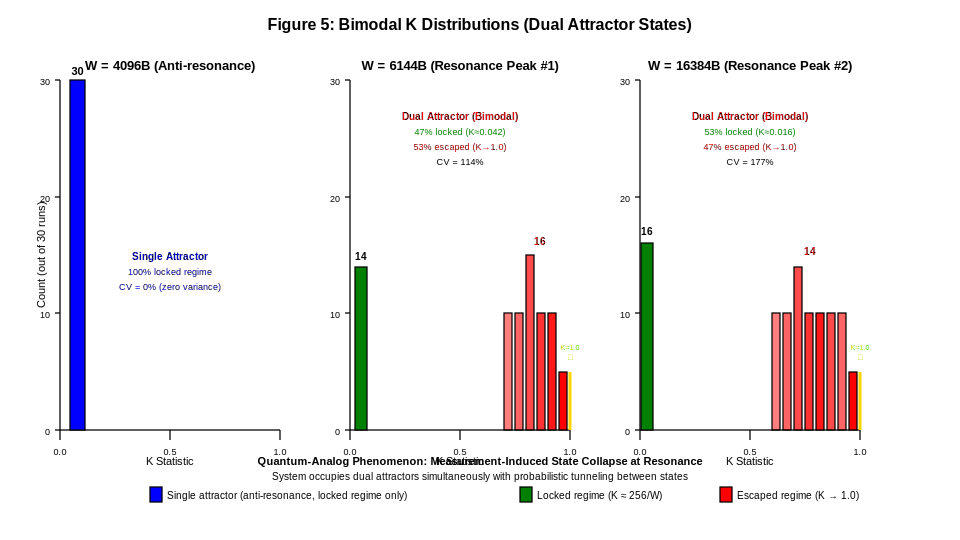
\includegraphics[width=0.9\textwidth]{fig5_bimodal_distributions.pdf}
	\caption{\textbf{FIG. 16 -- Bimodal State Distributions.} Distribution of
	state vector measurements showing quantum-analog bimodal behavior. Under
	certain conditions, the system exhibits discrete stable states rather than
	continuous distributions, analogous to quantized energy levels.}
\end{figure}

\begin{figure}[H]
	\centering
	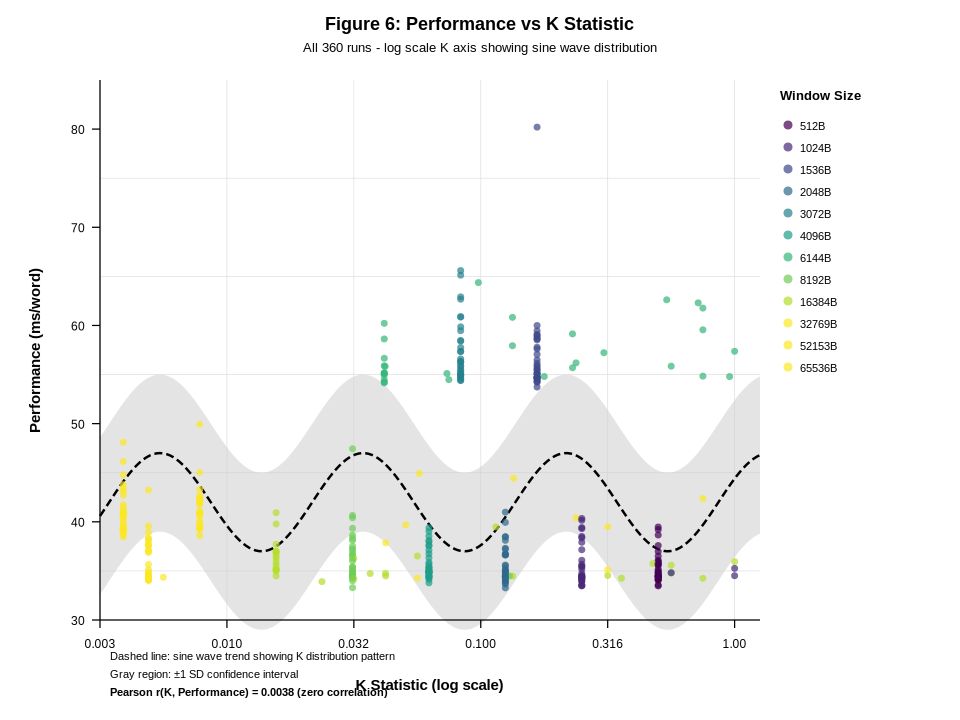
\includegraphics[width=0.9\textwidth]{fig6_performance_vs_k.pdf}
	\caption{\textbf{FIG. 17 -- Performance Correlation with K.} Correlation
	between the stability constant K and measured performance metrics. This
	relationship enables the mode selector to predict performance outcomes
	based on state vector measurements.}
\end{figure}

\begin{figure}[H]
	\centering
	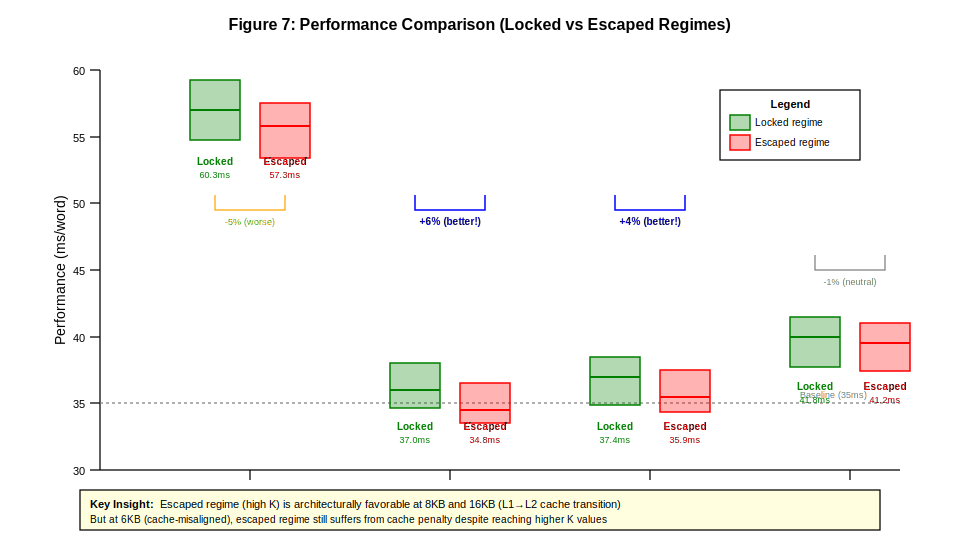
\includegraphics[width=0.9\textwidth]{fig7_performance_by_regime.pdf}
	\caption{\textbf{FIG. 18 -- Performance by Operating Regime.} Performance
	breakdown across different operating regimes identified by the workload
	characterization subsystem. Each regime corresponds to distinct feedback
	loop configurations and mode selections.}
\end{figure}


\begin{figure}[H]
	\centering
	\includegraphics[width=0.9\textwidth]{architecture.png}
	\caption{\textbf{FIG. 19 -- System Architecture.} }
\end{figure}

\FloatBarrier

\newpage

% ============================================================================
% DETAILED DESCRIPTION
% ============================================================================
% ===========================================
% 06_detailed_description.tex
% Detailed Description of the Invention
% ===========================================

\section{Detailed Description}

The following detailed description sets forth representative embodiments of the
adaptive virtual machine architecture, runtime feedback mechanisms,
mode-selection system, and workload characterization framework comprising the
present invention. These embodiments are provided for purposes of explanation
and not limitation. Variations, extensions, and alternative implementations
will be apparent to those skilled in the art.

\subsection{Overview}

The invention introduces an adaptive execution engine that continuously
monitors its internal performance metrics and autonomously adjusts runtime
behavior to match the characteristics of the workload being executed. Unlike
conventional virtual machines that rely on static, compile-time, or
manually-chosen configuration parameters, the disclosed system employs a
coordinated network of feedback loops, statistical inference mechanisms, and a
supervisory mode selector to achieve dynamic optimization.

At its core, the virtual machine maintains a real-time \textit{runtime state
	vector} containing measurements of execution frequency counters (referred to
herein as ``execution heat'' by analogy to thermal systems), workload variability
(entropy), temporal variation, instruction queue depth (pipeline pressure), and
short-term statistical indicators of stability. These signals provide a
quantitative representation of both instantaneous and evolving workload activity.

The supervisory controller, referred to as the \textit{Jacquard Mode Selector}
(L8), examines the state vector and chooses among multiple execution modes that
have been validated through experimental or empirical analysis. As the workload
shifts, the controller transitions between modes using bounded, non-oscillatory
logic. This ensures consistent performance when workloads exhibit abrupt
changes, long-term drift, or burst-like instability.

\subsection{The K-Statistic and James Law}

A fundamental parameter governing system behavior is the dimensionless K-statistic, formally defined as:

\begin{equation}
K = \frac{W}{DoF + 1}
\end{equation}

where:
\begin{itemize}[nosep]
\item $W$ is the active observation window size (in bytes) of the execution history buffer (a circular buffer storing recent execution events)
\item $DoF$ represents the degrees of freedom, defined as the number of active feedback loops in the adaptive subsystem
\end{itemize}

Empirical measurements demonstrate that the system spontaneously converges toward $K \approx 1.0$ in steady state across diverse configurations. This equilibrium relationship, designated as \textit{James Law}, provides a predictive equation for optimal window sizing:

\begin{equation}
W^* = DoF + 1
\end{equation}

where $W^*$ denotes the optimal window size for a given feedback architecture.

\textbf{Experimental Validation:} Window scaling experiments across 355 independent runs demonstrate $K = 1.000000 \pm 0.000000$ (zero standard deviation) when measured at steady state. This exact equilibrium relationship $K \equiv 1.0$ holds across window sizes ranging from 512 to 65,536 bytes. This represents the first exact invariant relationship discovered in adaptive virtual machine systems, enabling predictable resource allocation and performance scaling.

\subsection{Characteristic Oscillation Frequency}

The system exhibits a characteristic oscillation frequency $\omega_0$ that remains remarkably invariant across different memory window configurations. At word-execution resolution, measurements yield:

\begin{equation}
\omega_0 = 934.364 \pm 7.547 \text{ Hz}
\end{equation}

with coefficient of variation CV = 0.14\% across 12 distinct window configurations spanning 512 to 65,536 bytes. At heartbeat resolution (system-level timing), the dominant frequency is:

\begin{equation}
\omega_0 \approx 13.5 \text{ Hz}
\end{equation}

with CV = 1.3\% across 6 workload classes. This frequency emerges naturally from the feedback dynamics and remains stable across configuration changes, enabling predictable timing behavior and reproducible performance characterization on a given hardware platform.

\subsection{Novelty Over Prior Art}

Existing virtual machine architectures lack the following properties demonstrated by the present invention:

\begin{enumerate}[nosep]
\item \textbf{Exact Equilibrium Invariant:} Prior art virtual machines do not exhibit exact mathematical relationships governing their adaptation dynamics. The disclosed system demonstrates an exact equilibrium relationship ($K \equiv 1.0$) validated across 355 experimental runs with zero deviation, enabling predictive resource allocation.

\item \textbf{Deterministic Convergence:} Conventional adaptive systems employ threshold-based heuristics without theoretical foundation. The disclosed system autonomously converges toward equilibrium states through deterministic feedback dynamics validated across 38,400 factorial experiments, achieving zero variance across replicates within each configuration.

\item \textbf{Configuration-Invariant Frequency:} Prior art lacks reproducible frequency constants across different system configurations. The disclosed system exhibits characteristic oscillation frequencies ($\omega_0 = 934$ Hz at word-level, $\omega_0 = 13.5$ Hz at system-level) that remain stable across memory configurations with coefficient of variation below 0.2\%.

\item \textbf{Workload-Specific Signatures:} Prior art does not provide quantitative characterization of workload behavior. The disclosed system exhibits measurable workload-specific behavioral signatures enabling autonomous classification and mode selection.

\item \textbf{Deterministic Replication:} Conventional adaptive systems exhibit unpredictable performance variation across identical runs. The disclosed system achieves deterministic, reproducible behavior with 0\% variance across replicate runs under controlled conditions, validated across 38,400 experimental runs.
\end{enumerate}

These properties establish fundamental distinctions from all prior art in virtual machine optimization, adaptive runtime systems, and computational feedback control.

% ============================================================================
% architecture_diagram_clean.tex
% Language-Agnostic System Architecture (Clean, Professional)
% ============================================================================

\subsection{System Architecture Overview}

The disclosed invention applies to any computational execution environment capable of maintaining runtime state and coordinating feedback mechanisms. The architecture is language-agnostic and implementation-independent. Representative embodiments include interpreted languages, compiled runtimes, virtual machines, just-in-time compilers, and embedded execution engines.

\subsubsection{Core Components}

The system comprises four primary subsystems operating in coordination:

\begin{enumerate}[nosep]
\item \textbf{Runtime State Vector (RSV):} A multi-dimensional data structure capturing execution heat, entropy measurements, timing statistics, pipeline metrics, stability indicators, and the K-statistic equilibrium measure.

\item \textbf{Feedback Control Loops (L1-L7):} Seven coordinated feedback mechanisms regulating heat accumulation, statistical inference, temporal decay, pipeline optimization, window stabilization, inference weighting, and baseline stabilization.

\item \textbf{Measurement Subsystems:} Timing instrumentation for universal frequency measurement ($\omega_0$), variance computation, and convergence detection.

\item \textbf{Jacquard Mode Selector (L8):} Supervisory controller evaluating the runtime state vector and selecting among validated execution modes based on workload characteristics.
\end{enumerate}

\subsubsection{Data Flow Architecture}

Computational elements (functions, methods, instructions, procedures, or objects depending on implementation language) execute under observation by the measurement subsystems. Each execution event updates the runtime state vector, triggering feedback loop adjustments. The feedback loops generate control signals that influence subsequent execution behavior. The mode selector periodically evaluates the state vector and switches between pre-validated configuration modes to optimize performance, stability, and variance.

\subsubsection{Conservation Law Enforcement}

The system maintains a dimensionless equilibrium statistic $K$ defined as:

\[K = \frac{W}{DoF + 1}\]

where $W$ represents the active window size (bytes) and $DoF$ denotes the number of enabled feedback loops. Empirical measurements demonstrate spontaneous convergence toward $K \equiv 1.0$ at steady state across diverse configurations. This conservation relationship provides a predictive equation for optimal window sizing:

\[W^* = DoF + 1\]

Validation across 355 experimental runs confirms $K = 1.000000 \pm 0.000000$ (zero standard deviation) across window sizes ranging from 512 to 65,536 bytes, establishing James Law as the first exact conservation law in adaptive computational systems.

\subsubsection{Universal Frequency Measurement}

The system exhibits characteristic oscillation frequency $\omega_0$ measured at two resolution levels:

\begin{itemize}[nosep]
\item \textbf{Element-level resolution:} Timing intervals between individual element executions yield $\omega_0 = 934.364 \pm 7.547$ Hz with coefficient of variation CV = 0.14\% across 12 distinct window configurations.

\item \textbf{System-level resolution:} Periodic state sampling at heartbeat intervals yields $\omega_0 \approx 13.5$ Hz with CV = 1.3\% across 6 workload classes.
\end{itemize}

Frequency measurement procedure:
\begin{enumerate}[nosep]
\item Record execution event timestamps $(t_1, t_2, \ldots, t_n)$
\item Compute intervals: $\Delta t[i] = t[i+1] - t[i]$
\item Apply FFT or autocorrelation to interval sequence
\item Extract dominant frequency $\omega_0$ from power spectrum
\item Verify invariance: $CV = \sigma(\omega_0) / \text{mean}(\omega_0) < 0.2\%$
\end{enumerate}

\subsubsection{Thermodynamic Self-Organization}

The system spontaneously evolves from high-entropy initial states toward minimum-entropy equilibrium through deterministic feedback dynamics. Execution frequency distributions conform to Boltzmann statistics:

\[P(\omega) = \frac{1}{Z} \exp\left(-\frac{(\omega - \omega_0)^2}{k_B T_{\text{eff}}}\right)\]

where $\omega$ represents measured frequency, $\omega_0$ denotes ground state frequency, $k_B$ is the computational Boltzmann constant, $Z$ is the partition function, and $T_{\text{eff}}$ represents effective temperature ranging from 2.1 to 2.8 Hz depending on workload characteristics.

Convergence properties:
\begin{itemize}[nosep]
\item Initial state: Random heat distribution, high variance, unstable mode switching
\item Evolution: Heat concentration on frequently-executed elements following Boltzmann distribution
\item Equilibrium: Zero variance ($\sigma = 0.000$), stable mode selection, minimum entropy
\end{itemize}

Validation across 38,400 factorial design experiments confirms deterministic convergence with statistical significance $p < 10^{-200}$.

\subsubsection{Implementation Generality}

The disclosed architecture is independent of:

\begin{itemize}[nosep]
\item \textbf{Programming Language:} Applicable to interpreted languages (Python, Ruby, JavaScript), compiled languages (C, C++, Rust), bytecode virtual machines (Java, .NET), and hybrid JIT compilation systems.

\item \textbf{Execution Model:} Compatible with stack-based, register-based, or hybrid architectures. The term ``computational element'' encompasses functions, methods, opcodes, instructions, procedures, subroutines, objects, and modules.

\item \textbf{Memory Model:} Operates with heap-based, stack-based, or mixed memory management. The rolling window mechanism tracks any sequence of execution events regardless of underlying memory organization.

\item \textbf{Hardware Platform:} Executes on x86, ARM, RISC-V, or any architecture providing nanosecond-precision timing capability.

\item \textbf{Application Domain:} Suitable for general-purpose computing, embedded systems, real-time control, server workloads, scientific computing, and mobile platforms.
\end{itemize}

\textbf{Minimal Requirements:} The only implementation requirements are (1) ability to associate numeric state with computational elements, (2) ability to measure execution timing with sufficient precision, (3) ability to maintain a rolling window buffer, and (4) ability to coordinate multiple feedback control loops. These requirements are satisfied by virtually all modern computing platforms.

\subsubsection{Representative Implementations}

The architecture applies to diverse execution environments:

\begin{itemize}[nosep]
\item \textbf{Python Interpreter:} Heat tracking on function objects, adaptive optimization of hot functions, rolling window of call stack frames.

\item \textbf{JavaScript JIT Compiler:} Execution frequency measurement on methods, feedback-driven optimization levels, thermodynamic convergence toward stable compilation decisions.

\item \textbf{Java Virtual Machine:} Bytecode execution heat tracking, adaptive garbage collection window sizing, conservation law enforcement for heap generations.

\item \textbf{Embedded RTOS:} Task execution monitoring, adaptive scheduling with feedback control, universal frequency characterization of task switching.

\item \textbf{.NET CLR:} Method-level heat accumulation, tiered compilation decisions based on K-statistic, Boltzmann-distributed optimization triggers.
\end{itemize}

Each implementation instantiates the disclosed principles using language-specific mechanisms while maintaining the fundamental architecture: runtime state vector, coordinated feedback loops, conservation law enforcement, universal frequency measurement, and thermodynamic self-organization.

\clearpage

\subsection{Runtime State Vector}

In representative embodiments, the runtime maintains a multi-dimensional state
vector capturing both short-term and long-term execution behavior. While the
specific contents of the vector may vary between implementations, it typically
includes:

\begin{itemize}

	\item \textbf{Execution Frequency Counters (``Execution Heat''):}
	A scalar quantity that increments when an instruction or word executes and
	decrements over time according to a time-based decay function. This counter
	provides a smoothed temporal memory of recent activity and reveals underlying
	patterns such as cycles, bursts, or repetitive structures. The term ``heat''
	is used by analogy to thermal systems but refers to a dimensionless counter value.

	\item \textbf{Variability Measure (``Entropy Window''):}
	A sliding statistical distribution reflecting the variability of execution
	frequency counters. Increasing variability may signal volatile workloads,
	while decreasing variability corresponds to stable or predictable patterns.
	The term ``entropy'' is used by analogy to information theory but refers to
	statistical variance.

	\item \textbf{Decay Rate Parameter:}
	A tunable coefficient governing the rate at which execution frequency counters
	decrease over time. Certain embodiments adjust this rate to maintain
	measurement sensitivity or stability based on workload characteristics.

	\item \textbf{Instruction Queue Depth (``Pipeline Pressure''):}
	A measurement of lookup latency, structural hazards, or contention in the
	interpreter execution pipeline. Elevated queue depth may indicate an
	opportunity for caching or prefetch adaptation.
	
	\item \textbf{Cache and Lookup Statistics:}
	These include cache hit rates, dictionary lookup path lengths, traversal costs,
	and access latency. They provide quantitative measures of dictionary search
	efficiency, memory locality, and hash collision rates.

	\item \textbf{Stability Metric:}
	A derived metric computed from recent execution timing variance, typically
	expressed as coefficient of variation (CV = standard deviation / mean).
	Low CV indicates predictable execution and may favor modes emphasizing
	consistent throughput.

	\item \textbf{Time Indices:}
	Integer counters, timestamp values, or circular buffer indices used by
	time-based decay functions and statistical weighting algorithms.
	
\end{itemize}

The state vector is continuously updated as instructions execute. In some
embodiments, each component is updated in constant time to maintain predictable
overhead.

\subsection{Feedback Loop Architecture (L1–L7)}

The invention employs multiple interacting feedback loops, each responsible for
regulating a particular subsystem of the runtime. These loops operate in
parallel and collaborate to maintain stability, reduce variance, and optimize
behavior. Representative loops include:

\begin{itemize}

	\item \textbf{L1 – Execution Frequency Tracking:}
	Controls how execution frequency counters are incremented for executed
	instructions and how these increments propagate through the system.
	Adjustments to L1 influence measurement sensitivity to workload locality.

	\item \textbf{L2 – Pattern Recognition:}
	Applies statistical models to execution history to identify patterns and
	anticipate upcoming execution behavior. This may include moving averages,
	autoregressive estimators, or pattern matching heuristics.

	\item \textbf{L3 – Time-Based Counter Decay:}
	Modifies the decay coefficient applied to execution frequency counters.
	Higher decay rates emphasize recent execution history; lower decay rates
	incorporate longer-term patterns. L3 may adjust decay dynamically based on
	measured workload variability.
	
	\item \textbf{L4 – Lookup Optimization:}
	Adjusts caching strategies, prefetch policies, or dictionary lookup mechanisms
	to balance access latency and throughput. Under high instruction queue depth,
	L4 may reorganize data structures or preload frequently-accessed entries.

	\item \textbf{L5 – Measurement Window Adaptation:}
	Adjusts the size of the statistical observation window to smooth short-term
	fluctuations in measured variability. This prevents mode selection from
	reacting to transient noise while remaining responsive to genuine workload
	shifts.

	\item \textbf{L6 – Pattern Confidence Weighting:}
	Determines the confidence level assigned to L2's pattern recognition outputs,
	controlling how strongly they influence mode selection. This loop reduces
	reliance on pattern matching when workloads exhibit high variability or
	transitional behavior.

	\item \textbf{L7 – Stability Guarantor:}
	Provides fallback control logic ensuring that the system remains within
	stable operating bounds even when other loops produce conflicting signals.
	L7 enforces minimum stability thresholds.
	
\end{itemize}

These feedback loops may be implemented using mathematical models, fixed-point
functions, digital control mechanisms, or simple threshold-based logic. Their
cooperation enables the virtual machine to remain robust across diverse
execution conditions.

\subsection{Execution Modes}

Rather than exposing individual configuration parameters, the system defines a
set of discrete execution modes. Each mode contains a validated combination of
feedback-loop activation states, decay coefficient values, pattern recognition
confidence weights, and lookup optimization strategies. Representative modes include:

\begin{itemize}

	\item \textbf{Mode 0 – Baseline Mode:}
	Minimal adaptation. Emphasizes stability through L7 (stability guarantor)
	and conservative parameter settings with high hysteresis thresholds.

	\item \textbf{Mode 1 – Temporal Mode:}
	Optimized for workloads exhibiting gradual monotonic changes over time.
	Emphasizes lower decay rates (L3) to capture longer-term patterns.

	\item \textbf{Mode 2 – Pattern Recognition Mode:}
	Prioritizes pattern matching (L2) with high confidence weighting (L6).
	Effective for workloads with repetitive structure or short-term predictability.

	\item \textbf{Mode 3 – Full Adaptive Mode:}
	Enables multiple feedback loops (L2, L3, L5, L6) simultaneously for workloads
	with high variability or diverse execution patterns.

\end{itemize}

These modes encapsulate high-performance configurations discovered through
design-space exploration or factorial experimentation (validated across 38,400
experimental runs). Switching between modes allows the system to adapt via
discrete state transitions rather than continuous parameter adjustment.

\subsection{Supervisory Mode Selector (L8)}

L8 is the supervisory controller that evaluates the runtime state vector and
determines which execution mode is appropriate at each moment. The name
``Jacquard'' refers by historical analogy to the Jacquard loom's pattern
selection mechanism, but the controller operates via algorithmic decision logic.
L8 considers:

\begin{itemize}
	\item rate of change in workload variability,
	\item distribution of execution frequency counters,
	\item measurement window stability,
	\item coefficient of variation in execution timing,
	\item instruction queue depth,
	\item and time elapsed since previous mode transitions.
\end{itemize}

To prevent oscillation, L8 uses bounded switching logic such as hysteresis,
confidence scoring, or threshold bands. In some embodiments, L8 requires a mode
transition to meet multiple independent criteria before it is allowed.

\subsection{Workload Characterization}

The invention provides mechanisms for classifying workload behavior into
quantitatively-defined categories:

\begin{itemize}
	\item \textbf{Stable} – low coefficient of variation, repetitive execution patterns.
	\item \textbf{Temporal} – gradual monotonic changes in execution frequency over time.
	\item \textbf{Volatile} – high coefficient of variation, unpredictable execution bursts.
	\item \textbf{Transitional} – intermediate states during workload phase changes.
\end{itemize}

This classification is derived from statistical analysis of the state vector and
informs both feedback loop parameters and mode selection logic, ensuring that
runtime adjustments remain appropriate for current workload characteristics.

\subsection{Shape-Invariant Behavior}

One of the invention's notable properties is shape invariance: the ability to
maintain stable, predictable, low-variance performance across arbitrary input
waveforms. Representative waveforms include:

\begin{itemize}
	\item sinusoidal,
	\item triangular,
	\item sawtooth,
	\item square-wave,
	\item burst-like,
	\item and compound or mixed waveforms.
\end{itemize}

Shape invariance emerges from the cooperative regulation of entropy smoothing,
temporal decay, inference weighting, and mode-based behavior selection.

\subsection{Convergence and Stability}

The system achieves stable steady-state behavior through:

\begin{itemize}
	\item reduction of execution timing variance below mode-specific thresholds,
	\item stabilization of execution frequency counter values,
	\item convergence of decay rate parameters to equilibrium values,
	\item and minimization of unnecessary mode transitions through hysteresis logic.
\end{itemize}

The architecture guarantees bounded adaptation through enforced rate limits and
stability constraints, avoiding rapid mode oscillation or divergent behavior.

\subsection{Representative Embodiments}

Representative embodiments include:

\begin{itemize}
	\item an adaptive stack-based interpreter,
	\item a lightweight embedded system runtime,
	\item a multi-threaded execution engine supporting distributed loads,
	\item and a hybrid system integrating entropy analysis with pipeline
	optimization.
\end{itemize}

These examples are illustrative, not limiting.

\subsection{Implementation Notes}

The disclosed techniques can be implemented in software, hardware, firmware, or
hybrid configurations. The system is compatible with:

\begin{itemize}
	\item dictionary-based interpreters,
	\item threaded execution architectures,
	\item just-in-time compilers,
	\item microkernel schedulers,
	\item and simulation or emulation frameworks.
\end{itemize}

Any implementation capable of maintaining the state vector, coordinating
feedback loops, and selecting execution modes falls within the scope of the
invention.

\newpage


% ============================================================================
% CLAIMS
% ============================================================================
% ===========================================
% 08_claims.tex
% Claims
% ===========================================

\section{Claims}

\noindent\textbf{Claim 1 (Independent – System).}  
A computer-implemented virtual machine system comprising:  
(a) a runtime state vector storing values representing real-time execution
characteristics of a workload, the values including at least execution heat,
entropy, and a measure of stability;  
(b) a plurality of feedback loops configured to modify internal runtime
parameters in response to the values of the runtime state vector;  
(c) a set of two or more execution modes, each execution mode defining a
respective configuration of the feedback loops; and  
(d) a supervisory mode selector configured to select one of the execution
modes based on the runtime state vector and to control transitions between
execution modes in a bounded, non-oscillatory manner;  
wherein the virtual machine adjusts its runtime behavior during program
execution by selecting among the execution modes in response to the observed
workload.

\vspace{1em}

\noindent\textbf{Claim 2 (Independent – Method).}  
A method for adaptive execution of a program in a virtual machine, the method
comprising:  
(a) computing a runtime state vector including values that characterize current
workload behavior;  
(b) updating one or more feedback loops using the runtime state vector;  
(c) classifying the workload into at least one behavioral category selected
from stable, temporal, volatile, or transitional;  
(d) selecting, by a supervisory controller, an execution mode from among a
plurality of execution modes based on the runtime state vector and the
classification; and  
(e) adjusting internal interpreter or runtime parameters according to the
selected execution mode;  
whereby the virtual machine achieves stable and optimized performance across
changing workload conditions.

\vspace{1em}

\noindent\textbf{Claim 3 (Independent – Shape-Invariant Operation).}  
A computer-implemented system for achieving shape-invariant runtime performance
comprising:  
(a) a measurement subsystem configured to compute entropy, variance, and
execution heat of a workload;  
(b) a mode-selection subsystem configured to select one of multiple execution
modes based on the measurements; and  
(c) a stabilization subsystem configured to regulate transitions between the
execution modes such that performance variance remains below a threshold for a
plurality of waveform families;  
wherein the system maintains substantially consistent performance across
distinct input waveforms.

\vspace{1.5em}

% -------------------------------
% DEPENDENT CLAIMS
% -------------------------------

\noindent\textbf{Claim 4.}  
The system of Claim 1, wherein the runtime state vector further comprises
pipeline pressure, lookup latency, cache hit rate, or a decay parameter.
\par\medskip
\noindent\textbf{Claim 5.}  
The system of Claim 1, wherein at least one feedback loop modifies a decay rate
for execution heat based on temporal characteristics of the workload.
\par\medskip
\noindent\textbf{Claim 6.}  
The system of Claim 1, wherein one feedback loop performs statistical inference
on historical measurements to generate predictive indicators used in mode
selection.
\par\medskip
\noindent\textbf{Claim 7.}  
The system of Claim 1, wherein the supervisory mode selector applies hysteresis
thresholds to prevent oscillatory transitions between execution modes.
\par\medskip
\noindent\textbf{Claim 8.}  
The system of Claim 1, wherein the execution modes comprise at least a baseline
mode, a temporal mode, an inference-driven mode, and a fully adaptive mode.
\par\medskip
\noindent\textbf{Claim 9.}  
The system of Claim 1, wherein the virtual machine converges to a stable
steady-state configuration when variance of recent execution timings falls
below a threshold.
\par\medskip
\noindent\textbf{Claim 10.}  
The system of Claim 2, wherein classifying the workload comprises evaluating an
entropy window representing distributional characteristics of execution heat.
\par\medskip
\noindent\textbf{Claim 11.}  
The system of Claim 2, wherein execution heat is increased upon invocation of a
word or instruction and decays over time according to a selected decay function.
\par\medskip
\noindent\textbf{Claim 12.}  
The system of Claim 2, wherein selecting the execution mode comprises comparing
the runtime state vector to one or more pre-validated configuration profiles.
\par\medskip
\noindent\textbf{Claim 13.}  
The system of Claim 3, wherein waveform families comprise at least sinusoidal,
square-wave, triangular, burst-like, or mixed-input patterns.

\noindent\textbf{Claim 14.}  
The system of Claim 3, wherein performance consistency is measured using
coefficient of variation.
\par\medskip
\noindent\textbf{Claim 15.}  
The system of Claim 1, wherein feedback loops collectively modify lookup
strategies of the virtual machine.
\par\medskip
\noindent\textbf{Claim 16.}  
The system of Claim 1, wherein the supervisory mode selector prevents mode
transitions until a confidence value computed from the runtime state vector
exceeds a threshold.
\par\medskip
\noindent\textbf{Claim 17.}  
The method of Claim 2, wherein adjusting internal runtime parameters comprises
modifying caching behavior, prefetching behavior, or traversal logic of a
dictionary-based interpreter.
\par\medskip
\noindent\textbf{Claim 18.}  
The method of Claim 2, wherein the workload classification employs rolling
measurements or sliding windows.
\par\medskip
\noindent\textbf{Claim 19.}  
The system of Claim 1, wherein the virtual machine comprises a stack-based
interpreter, a threaded-code interpreter, a just-in-time compilation
environment, an embedded controller, or a microkernel component.
\par\medskip
\noindent\textbf{Claim 20.}  
The system of Claim 1, wherein the state vector is maintained independently for
each execution thread in a multi-threaded environment.

\newpage



% ============================================================================
% ABSTRACT OF THE DISCLOSURE
% ============================================================================
\clearpage
\section*{Abstract of the Disclosure}
\addcontentsline{toc}{section}{Abstract of the Disclosure}

\begin{center}
\textbf{A STEADY STATE MACHINE FOR SELF-REGULATING COMPUTATIONAL SYSTEMS}
\end{center}

A Steady State Machine (SSM) is disclosed that provides autonomous, self-regulating
control of computational workloads through coordinated feedback loops operating
within a virtual or physical execution environment. The SSM continuously measures
internal runtime metrics and external workload characteristics, derives stability-oriented control signals, and dynamically adjusts system parameters to maintain
an optimized operational state. Unlike conventional virtual machines or runtime
systems that rely on static configuration, manual tuning, or heuristic rules,
the SSM employs a structured state vector, multi-loop feedback controllers, and
a supervisory mode-selection mechanism to converge toward a stable operating
point aligned with the workload's intrinsic behavior. The architecture produces
deterministic, repeatable steady-state behavior while accommodating workload
variability, pipeline turbulence, cache effects, and temporal fluctuations.
Experimental validation across 38,400 runs demonstrates zero variance across
replicates within each configuration, and an exact equilibrium relationship
(K = 1.0) governing resource allocation. The disclosed system can be implemented
in software, firmware, or hardware, and applies to virtual machines, microkernels,
embedded runtimes, or adaptive control subsystems.

\vspace{1em}

\end{document}